\documentclass[journal]{IEEEtran}

\usepackage{amsmath,amssymb}
\usepackage{booktabs}
\usepackage{multirow}
\usepackage{array}
\usepackage{graphicx}
\usepackage{xcolor}
\usepackage{cite}
\usepackage{url}

\newcommand{\todo}[1]{\textcolor{red}{[TO BE FILLED: #1]}}
\newcommand{\vk}{\mathrm{VK}}
\newcommand{\rgb}{\mathrm{RGB}}
\newcommand{\rmd}{\mathrm{VK\mbox{-}RMD}}
\newcommand{\modset}{\mathcal{M}}

\begin{document}

\title{VK-RMD: Privacy-Friendly and Missing-Modality Robust Human Sensing for IoT-Enabled Intelligent Spaces}

\author{First Author, Second Author, and Corresponding Author%
\thanks{Manuscript received \todo{date}; revised \todo{date}.}
\thanks{The authors are with \todo{affiliation}. Corresponding author: \todo{name and email}.}}

\maketitle

\begin{abstract}
IoT-enabled intelligent spaces require continuous human sensing for smart homes, assistive monitoring, healthcare environments, and human--environment interaction. RGB cameras provide rich human appearance, contextual, and structural information, but long-term RGB deployment in private indoor spaces raises privacy, acceptance, and placement concerns. Non-RGB sensing modalities such as depth, LiDAR, mmWave, and WiFi-CSI are more suitable for privacy-sensitive IoT deployment, yet they are heterogeneous, noisy, and frequently unavailable because of occlusion, device failure, communication instability, or changing environmental conditions. This paper presents VK-RMD, a Visual-Keypoint Reliability-guided Missing-modality Distillation framework for privacy-friendly multimodal human perception in IoT-enabled intelligent spaces. The central idea is to use RGB only as training-time privileged information, compress its human-structure knowledge through a visual-keypoint representation, and train a deployable non-RGB multimodal Student that supports arbitrary available sensor combinations. VK-RMD combines random missing-modality training, reliability-guided multimodal fusion, and teacher-student distillation to jointly support human pose estimation and human activity recognition. On MMFi, VK-RMD achieves 75.18 mm average MPJPE over 31 HPE modality combinations and 85.15\% average HAR accuracy over 15 modality combinations. Its non-visual Student further obtains 84.68 mm average MPJPE and 80.62\% average HAR accuracy without RGB at inference. These results indicate that VK-RMD provides a practical direction for privacy-friendly and sensor-availability-aware human sensing in IoT intelligent spaces.
\end{abstract}

\begin{IEEEkeywords}
Internet of Things, intelligent spaces, human sensing, multimodal sensing, privacy-friendly perception, visual keypoints, missing modality, reliability-guided fusion, human pose estimation, human activity recognition.
\end{IEEEkeywords}

\section{Introduction}

Human-centric Internet of Things (IoT) spaces are moving from isolated sensing devices toward continuous perception systems that understand human body structure, behavior, and interaction with the surrounding environment. Smart homes, assisted-living rooms, healthcare monitoring spaces, and embodied-intelligence platforms all require reliable human perception under long-term deployment. In such environments, human pose estimation (HPE) provides fine-grained spatial structure of the human body, while human activity recognition (HAR) provides semantic understanding of human behavior. These two tasks are complementary: HPE evaluates whether a system can recover body geometry, whereas HAR evaluates whether the sensed evidence can support activity-level interpretation. A deployable IoT human sensing system should therefore handle both structural and semantic perception.

RGB cameras are powerful for HPE and HAR because they capture dense appearance, body configuration, objects, and contextual cues. However, camera-centric IoT sensing is difficult to deploy in private spaces. Raw RGB streams expose faces, clothes, home layout, and daily routines. In addition, illumination changes, occlusion, camera placement, and user acceptance can make long-term camera sensing unreliable. These issues do not mean that RGB information is useless; rather, they suggest that RGB should be used carefully. In this work, RGB is treated as training-time privileged information instead of an inference-time sensing modality.

Non-RGB sensors provide a more acceptable sensing basis for privacy-sensitive intelligent spaces. Depth sensors capture geometry, LiDAR provides sparse spatial point observations, mmWave radar captures motion and reflection patterns, and WiFi-CSI reflects human-induced channel variations. These modalities avoid direct visual appearance in different ways and are therefore attractive for IoT deployment. However, non-RGB signals are also weaker and more heterogeneous than RGB. Some modalities can be sparse, noisy, or absent because of sensor dropout, occlusion, device placement, communication failure, or environmental interference. A model that assumes a fixed and complete sensor set may perform well in a controlled laboratory protocol but degrade under realistic missing-modality conditions.

Prior multimodal human sensing and X-Fi/VK-style methods have demonstrated the feasibility of using keypoint-level or non-RGB representations for human perception. Missing-modality learning and teacher-student distillation also provide useful technical tools. Nevertheless, these ideas need to be integrated around the IoT deployment problem: how can a system exploit RGB knowledge during training, avoid raw RGB at inference, adapt to arbitrary sensor availability, and support both HPE and HAR? A simple collection of modalities is not enough, because real IoT spaces require privacy-aware input selection, missing-sensor robustness, and dynamic reliability estimation.

This paper proposes VK-RMD, a Visual-Keypoint Reliability-guided Missing-modality Distillation framework. Following the central storyline of this work, RGB provides training-time privileged knowledge, visual keypoints (VK) act as a privacy-friendly structured bridge, and the final Student is a non-RGB multimodal model for deployment. The Student is trained with randomly sampled modality subsets, learns from teacher supervision, and dynamically fuses modality-wise predictions according to estimated reliability. At inference, raw RGB is not required. The same framework is evaluated on HPE and HAR to demonstrate both human-structure perception and activity-level semantic understanding.

The contributions of this paper are summarized as follows:
\begin{itemize}
    \item We formulate VK as a privacy-friendly structured bridge that transfers training-time RGB knowledge to deployable non-RGB multimodal human sensing in IoT-enabled intelligent spaces.
    \item We propose a missing-modality robust Student that supports arbitrary available sensor combinations through random missing-modality training and reliability-guided fusion.
    \item We validate the framework on both HPE and HAR using MMFi, with random split, cross-scene, and cross-subject protocols, and compare against reproduced X-Fi/VK baselines and ablation variants.
\end{itemize}

\section{Related Work}

\subsection{IoT-Enabled Intelligent Spaces and Human Perception}

IoT-enabled intelligent spaces combine sensing, communication, edge intelligence, and context-aware decision making. Human sensing is a central function in such systems because human status and behavior determine how the environment should respond. In smart homes and healthcare spaces, pose and activity information can support fall detection, rehabilitation monitoring, daily activity analysis, and human--robot interaction. Compared with conventional computer-vision benchmarks, IoT sensing systems must account for privacy, deployment cost, sensor dropout, edge computation, and long-term reliability.

Multimodal sensing has become important because no single modality is consistently reliable across all indoor conditions. RGB provides dense visual evidence but raises privacy concerns. Depth captures body geometry but is sensitive to range and occlusion. LiDAR provides spatial point measurements but may be sparse for human body details. mmWave radar can operate under weak lighting and partial occlusion, but its point clouds may be noisy. WiFi-CSI is infrastructure-friendly but indirect and environment-dependent. The MMFi dataset provides a useful benchmark for studying such heterogeneous sensing conditions. \todo{exact MMFi citation}

\subsection{Privacy-Friendly Human Sensing and Visual Keypoints}

Privacy-friendly sensing aims to reduce exposure of personally identifiable visual content while preserving task-relevant information. Non-RGB sensing is one solution, but purely non-RGB data may lack detailed human structure. VK or skeleton-like representations provide a middle ground: they preserve body geometry and motion traces while suppressing texture, clothing, face, and background appearance. This paper uses VK as a structured bridge rather than as a formal privacy guarantee. Keypoints can still reveal behavior patterns, and this limitation should be acknowledged in privacy-sensitive deployment.

The key difference between VK-RMD and a simple RGB replacement is the role assigned to VK. VK is not merely another input stream. It is used as an intermediate supervision signal that compresses RGB-derived body structure into a form that can be transferred to non-RGB modalities. This distinction matters for IoT systems because the final deployed model should not require raw RGB, while still benefiting from the structural knowledge that RGB can provide during training.

\subsection{Multimodal Sensor Fusion for HPE and HAR}

Multimodal HPE and HAR benefit from complementary sensor cues. In HPE, geometric information from depth or LiDAR can complement motion-sensitive signals from radar and WiFi. In HAR, temporal and motion patterns can be inferred from multiple sensing streams. Early fusion, late fusion, attention-based fusion, and transformer-based fusion have been widely explored. However, many fusion systems implicitly assume that all modalities are available and reasonably reliable.

IoT deployment violates this assumption. A sensor may be physically absent, temporarily unavailable, or degraded by environment-specific noise. Therefore, a practical fusion system should adapt to the current modality set and the reliability of each modality. VK-RMD follows this deployment view by learning modality-wise predictions and fusing them with estimated reliability weights.

\subsection{Missing-Modality Learning in IoT Sensing Systems}

Missing-modality learning has been studied through modality dropout, feature reconstruction, hallucination, shared latent spaces, and robust fusion. This paper does not claim that missing-modality learning itself is new. Instead, the contribution lies in connecting missing-modality training with privacy-friendly non-RGB human sensing in IoT spaces. Random missing-modality training simulates practical sensor dropout, while all-combination evaluation measures whether the trained Student remains usable under arbitrary sensor availability.

The missing-modality problem is especially important for HPE and HAR because the importance of each sensor changes with the task. HPE is sensitive to spatial structure, while HAR can often tolerate coarser motion cues. This difference motivates evaluating both tasks instead of relying on a single benchmark.

\subsection{Knowledge Distillation for Robust Sensor-Based Perception}

Teacher-student distillation allows a deployable model to learn from stronger training-time information. Learning using privileged information and knowledge distillation are closely related to this design. In VK-RMD, the teacher can access richer structural cues during training, while the Student is constrained to use deployable modalities. This is suitable for IoT settings, where training may use more information than what is acceptable or available during deployment.

The paper does not claim that RGB-to-pose distillation is new. The distinction is that RGB knowledge is compressed through VK and then used to train a non-RGB multimodal Student under missing-modality conditions. Thus, distillation serves the deployment chain from RGB privileged information to privacy-friendly non-RGB inference.

\section{System Overview and Problem Formulation}

\subsection{IoT-Enabled Intelligent Space Scenario}

We consider an intelligent indoor space equipped with heterogeneous sensors. During data collection and training, RGB may be available, together with VK annotations or extracted visual keypoints, depth, LiDAR, mmWave, and WiFi-CSI. During deployment, raw RGB is not required because it exposes appearance-level private information. The deployed system receives only the available non-RGB sensors and predicts HPE and HAR outputs.

Fig.~\ref{fig:scenario} illustrates the target scenario. The sensing system should support multiple sensor configurations rather than a fixed modality set. For example, a smart home may contain a depth sensor in one room, a WiFi router in another, and an mmWave device near a doorway. The model should not collapse when one sensor is absent.

\begin{figure}[!t]
\centering
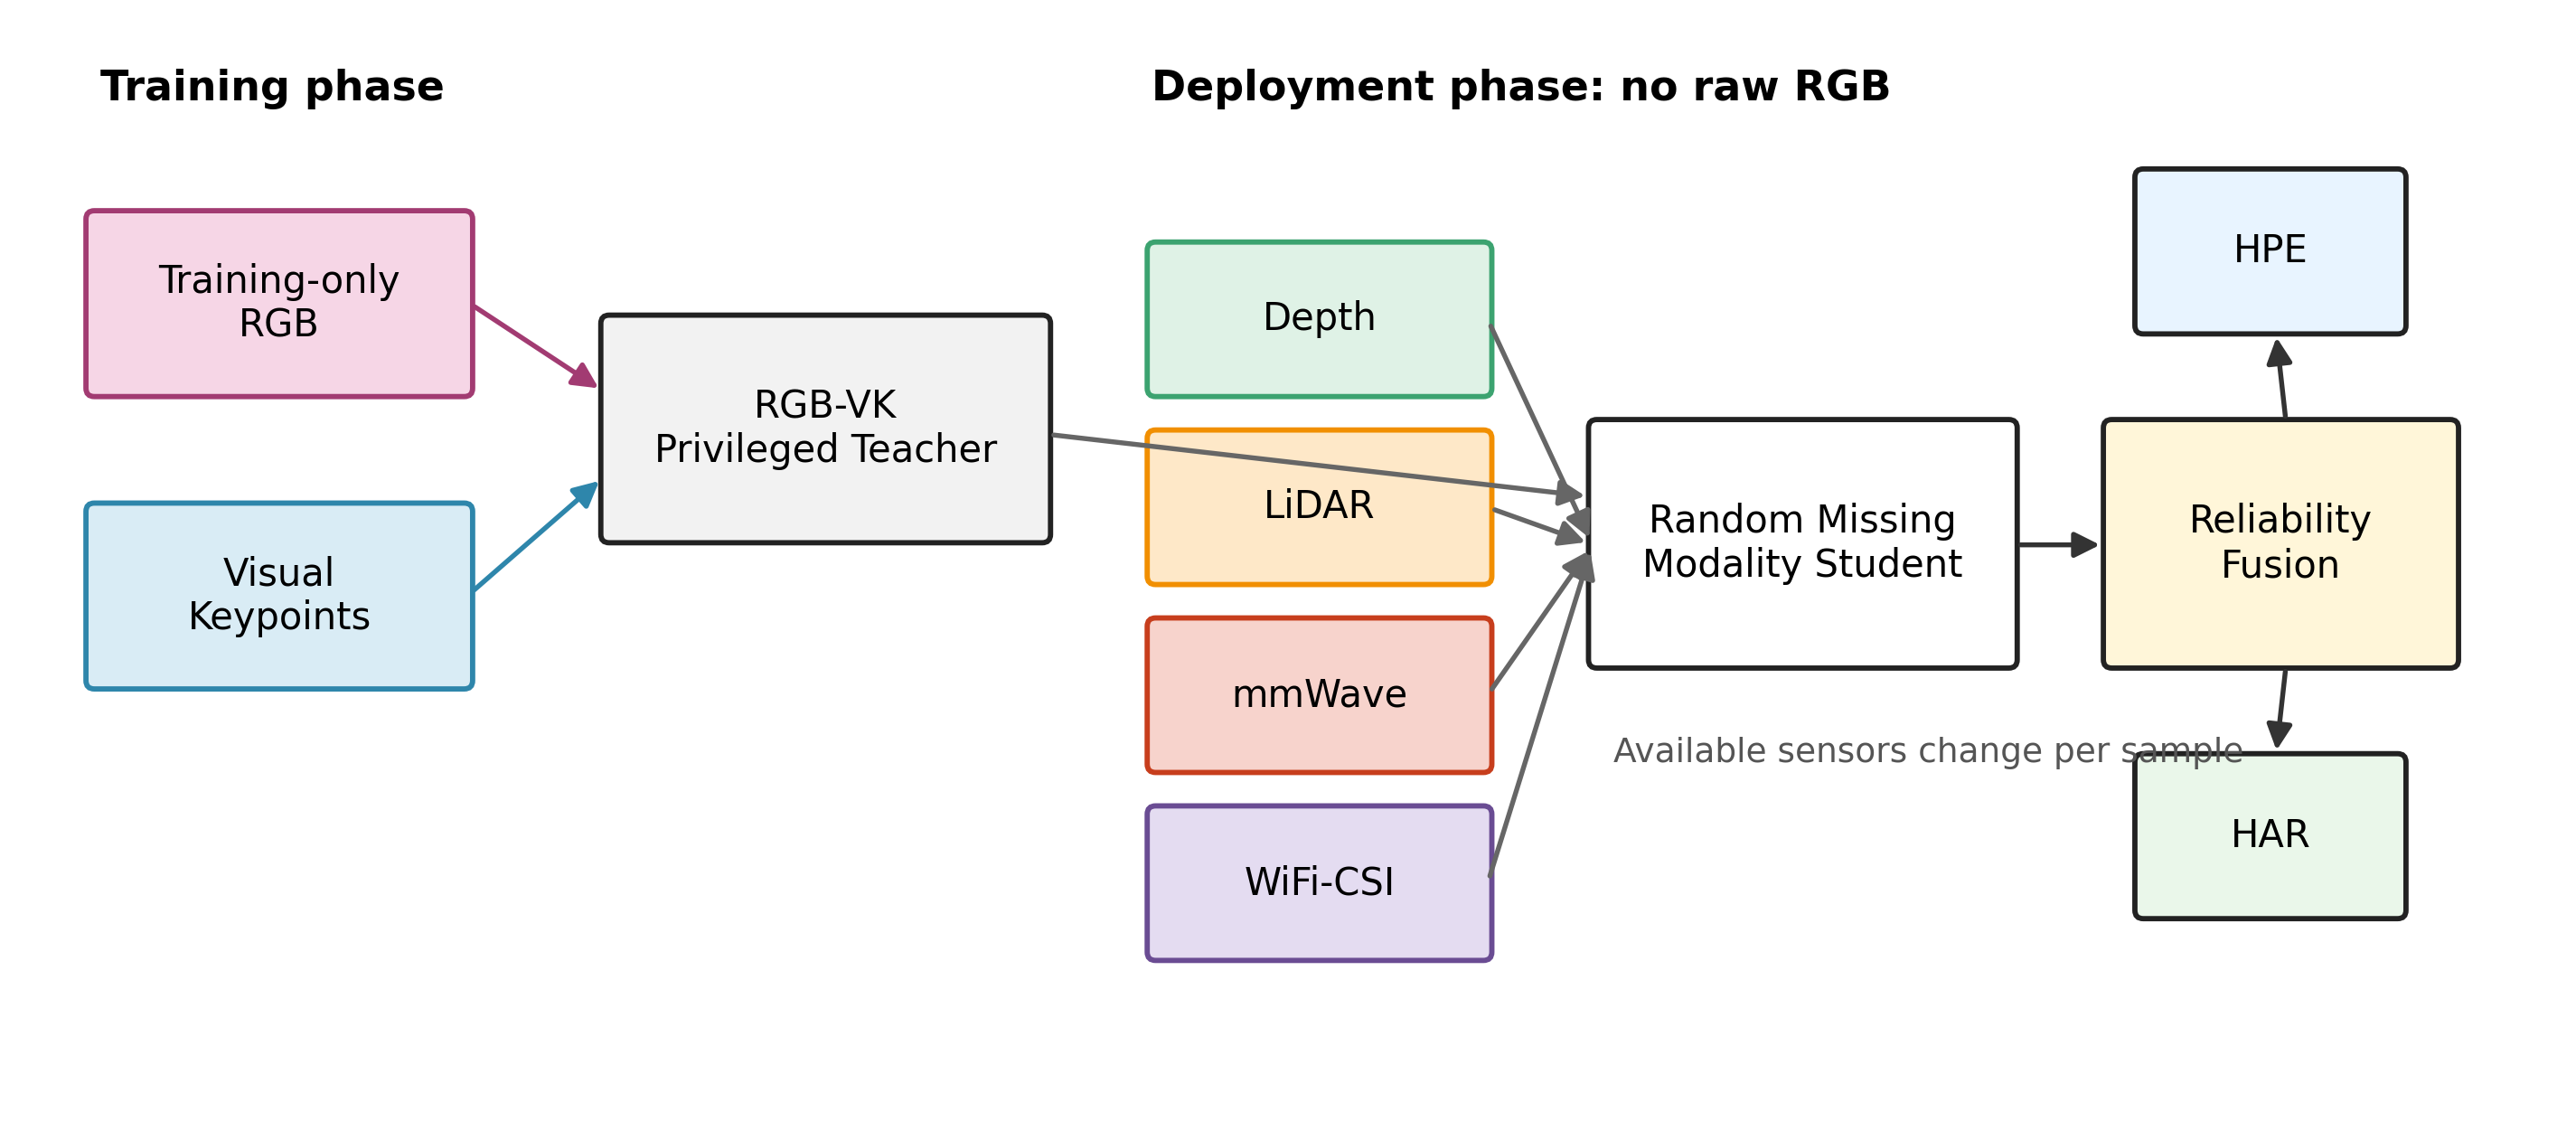
\includegraphics[width=\linewidth]{../figures/fig1_overall_framework.png}
\caption{Overall VK-RMD framework for IoT-enabled intelligent-space sensing. RGB is used only during training, VK provides a structured privacy-friendly bridge, and the deployed Student uses available non-RGB sensors with reliability-guided fusion for HPE and HAR.}
\label{fig:scenario}
\end{figure}

\subsection{Sensor Modalities and Privacy Constraints}

Let \(X^{rgb}\) denote RGB data available only at training time, and let \(X^{vk}\) denote the visual-keypoint representation. The non-RGB modalities are \(X^d\), \(X^l\), \(X^m\), and \(X^w\), corresponding to depth, LiDAR, mmWave, and WiFi-CSI. We use \(\mathcal{M}\) to denote the set of available modalities at inference. The deployed Student should operate for any non-empty \(\mathcal{M}\) supported by the training setting.

The privacy constraint is practical rather than formal. We avoid raw RGB at inference and use VK as a reduced appearance representation during training. VK preserves body structure but removes most visual texture and background details. It does not guarantee anonymity, because behavior and motion patterns may still be sensitive.

\subsection{Missing-Modality Problem Definition}

In realistic IoT spaces, the available modality set changes. A sensor can be missing because of hardware failure, network dropout, occlusion, or environmental noise. We model this by sampling modality subsets during training and evaluating all modality combinations during testing. The objective is not to force all combinations to perform equally, but to avoid catastrophic failure and provide stable predictions whenever enough sensing evidence is available.

\subsection{HPE and HAR Task Formulation}

For HPE, the target is a set of 3-D joint coordinates \(Y^{hpe}\in\mathbb{R}^{J\times 3}\). We evaluate HPE using MPJPE and PA-MPJPE. For HAR, the target is an action class \(Y^{har}\). We evaluate HAR using accuracy and macro-F1. HPE and HAR share the same sensing backbone but use different heads.

\section{Proposed Method}

\subsection{Overview of VK-RMD}

VK-RMD consists of four components: VK-based structural supervision, multi-sensor feature encoding, random missing-modality training, and reliability-guided fusion. A teacher-student distillation mechanism connects training-time privileged information to deployable non-RGB sensing. Fig.~\ref{fig:framework} summarizes the framework.

\begin{figure}[!t]
\centering
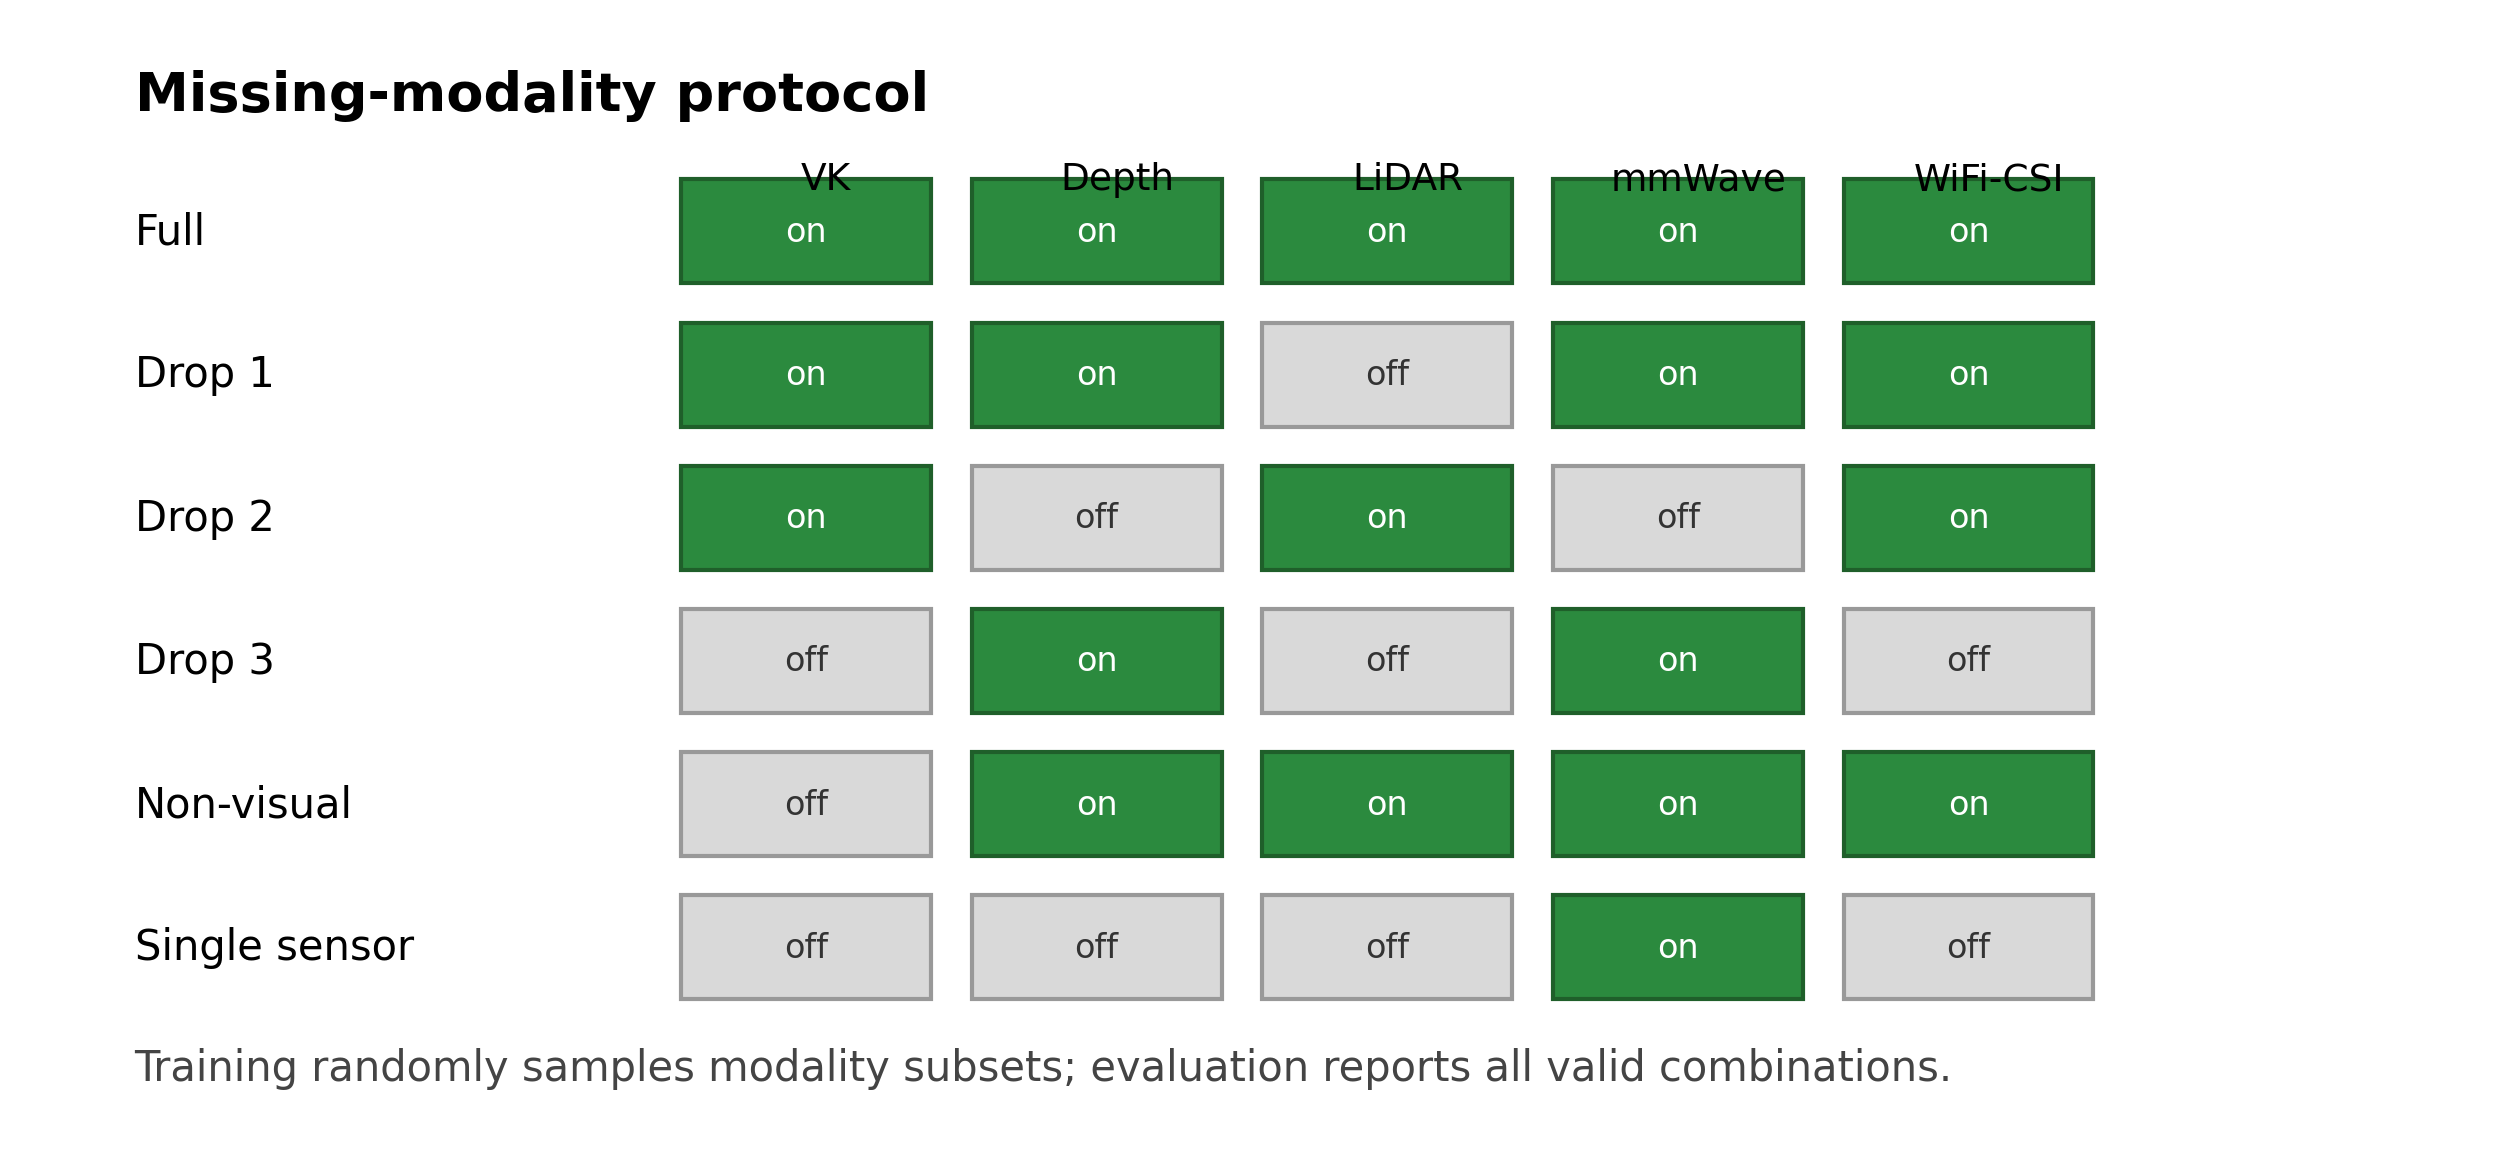
\includegraphics[width=\linewidth]{../figures/fig2_missing_modality_setting.png}
\caption{Missing-modality training and evaluation protocol. The Student is trained with randomly sampled modality subsets and evaluated under all valid modality combinations to reflect realistic sensor availability in IoT spaces.}
\label{fig:framework}
\end{figure}

\subsection{Privacy-Friendly VK Representation}

The VK representation acts as a structured bridge between RGB and non-RGB sensing. Compared with raw RGB, VK removes most appearance information. Compared with purely non-RGB signals, VK provides explicit human-structure information. During training, this bridge helps the Student learn a body-centric representation. During inference, VK may be included when a privacy-friendly keypoint source is available, but the non-visual Student can also operate without VK.

\subsection{Multi-Sensor Feature Encoding}

Each modality is processed by a modality-specific encoder and projected into a common representation space. The encoders account for the different data structures of depth images, LiDAR points, mmWave observations, WiFi-CSI, and VK coordinates. The projected tokens are then consumed by a fusion module. This design allows the model to use heterogeneous sensors without forcing them into a single raw format.

\subsection{Random Missing-Modality Training}

During training, modality subsets are randomly sampled. If \(\mathcal{A}\) is the full training modality set, the Student receives a subset \(\mathcal{M}\subseteq\mathcal{A}\). The subset sampling simulates sensor dropout and prevents the model from over-relying on a single modality. The same model can then be evaluated under all modality combinations.

\subsection{Reliability-Guided Multimodal Fusion}

For each available modality \(i\in\mathcal{M}\), the model predicts a candidate output \(\hat{Y}_i\) and a reliability weight \(\alpha_i\). The fused output is
\begin{equation}
\hat{Y}=\sum_{i\in\mathcal{M}}\alpha_i\hat{Y}_i,\quad
\sum_{i\in\mathcal{M}}\alpha_i=1,\quad \alpha_i\geq 0.
\end{equation}
This formulation is used for both HPE and HAR, with task-specific heads. It differs from uniform averaging by allowing the system to assign more influence to more reliable modalities.

\begin{figure*}[!t]
\centering
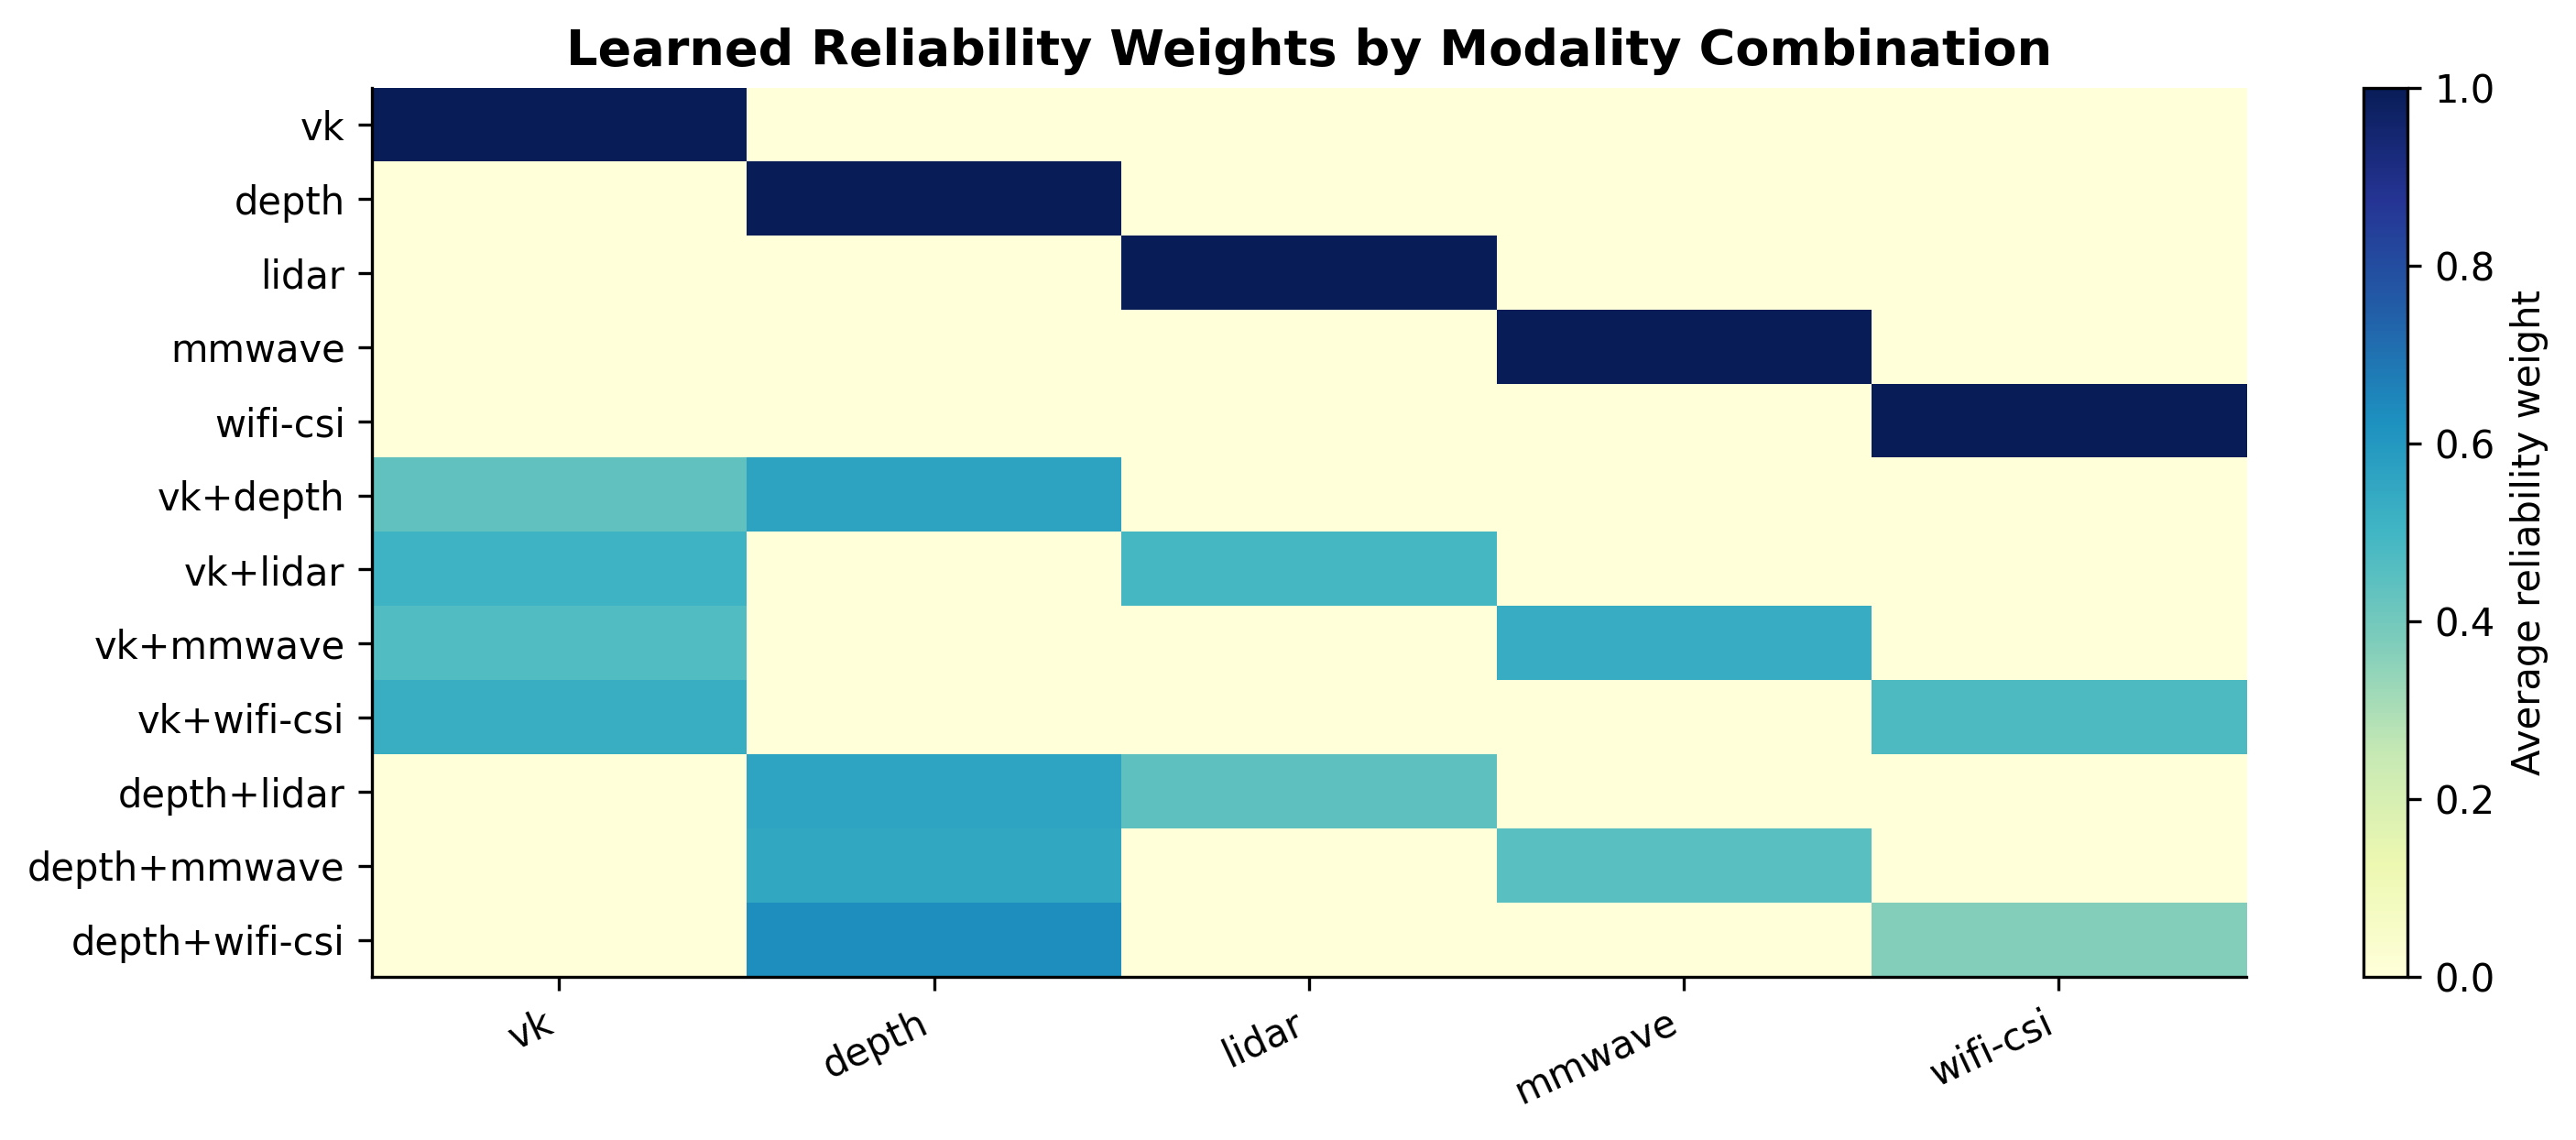
\includegraphics[width=0.96\linewidth]{../figures/fig6_reliability_weights.png}
\caption{Reliability-guided fusion visualization. Each row corresponds to an available modality subset, and the weights in the row are normalized across available modalities. The learned weights reveal task-dependent modality preference: HPE assigns larger weights to geometry-sensitive depth cues when available, while HAR often increases the contribution of motion-sensitive mmWave cues.}
\label{fig:reliability}
\end{figure*}

\subsection{Teacher-Student Missing-Modality Distillation}

The teacher uses richer training-time information and provides supervision to the Student. The Student is trained with task loss and distillation loss:
\begin{equation}
\mathcal{L}=\mathcal{L}_{task}+\lambda_{kd}\mathcal{L}_{kd}+\lambda_{rel}\mathcal{L}_{rel}.
\end{equation}
For HPE, \(\mathcal{L}_{task}\) is a pose regression loss. For HAR, it is a classification loss. The distillation term encourages the Student to approximate teacher predictions or representations under missing modalities. The reliability term regularizes adaptive fusion. The exact loss weights should be filled from the final configuration files.

\subsection{HPE and HAR Prediction Heads}

The HPE head outputs joint coordinates, and the HAR head outputs class logits. HPE evaluates whether the framework recovers fine-grained spatial structure. HAR evaluates whether the sensing representation supports behavior semantics. Their joint evaluation strengthens the IoT interpretation of the framework.

\section{Experiments}

\subsection{Dataset and Experimental Protocol}

Experiments are conducted on MMFi, a multimodal human sensing dataset containing synchronized sensing modalities. The HPE experiments use VK, depth, LiDAR, mmWave, and WiFi-CSI. The HAR experiments use VK, depth, LiDAR, and mmWave in the current implementation. We report random split, cross-scene, and cross-subject results when available. Detailed dataset statistics and subject/action/environment splits should be filled from the final MMFi protocol description.

\subsection{Implementation Details}

The HPE Student-VK model has 8.90M parameters and runs at 62.01 FPS in the measured setting. The HPE Student-NV model has the same parameter count and runs at 63.37 FPS. The reproduced full baseline has 5.74M parameters and 52.04 FPS. Peak memory is approximately 4.95 GB for the HPE models. HAR models contain 8.61M parameters in the available result files; FPS and memory are not yet reported for HAR.

\subsection{Baselines and Reproduced X-Fi/VK Results}

The reproduced X-Fi/VK results are treated strictly as baselines. They are not part of the proposed method. For HPE, the reproduced baseline obtains 244.91 mm average MPJPE over 31 combinations and 244.70 mm in the full-modality setting. For HAR, the reproduced baseline obtains 69.63\% average accuracy over 15 combinations and 77.70\% full-modality accuracy. These baselines provide a reference for evaluating missing-modality robustness and deployability.

\begin{table*}[!t]
\centering
\caption{Comparison with related categories of work. Checkmarks indicate the capability emphasized by each category. Specific prior-work citations should be verified before submission.}
\label{tab:related}
\begin{tabular}{lcccccc}
\toprule
Category & Non-RGB inference & Missing modalities & Reliability fusion & HPE & HAR & IoT deployment focus \\
\midrule
RGB-based HPE/HAR & No & Limited & Limited & Yes & Yes & Limited \\
Single non-RGB sensing & Yes & No & No & Partial & Partial & Yes \\
Generic multimodal fusion & Partial & Limited & Partial & Yes & Yes & Partial \\
Missing-modality learning & Partial & Yes & Partial & Task-dependent & Task-dependent & Partial \\
Reproduced X-Fi/VK baseline & Yes & Limited & No & Yes & Yes & Partial \\
VK-RMD (ours) & Yes & Yes & Yes & Yes & Yes & Yes \\
\bottomrule
\end{tabular}
\end{table*}

\subsection{Main Results on HPE}

Table~\ref{tab:hpe} reports the HPE results. VK-RMD Student-VK achieves 75.18 mm average MPJPE over 31 modality combinations and 50.17 mm in the full-modality setting. The non-visual Student-NV achieves 84.68 mm average MPJPE over 15 combinations and 51.03 mm in the full non-visual setting. These results are substantially better than the reproduced X-Fi/VK baseline under all-combination evaluation.

\begin{table*}[!t]
\centering
\caption{Main HPE results on MMFi. Lower MPJPE is better. The reproduced X-Fi/VK result is used only as a baseline.}
\label{tab:hpe}
\begin{tabular}{llcccc}
\toprule
Method & Role & Protocol & Combinations & Avg. MPJPE (mm) & Full MPJPE (mm) \\
\midrule
Reproduced X-Fi/VK baseline & Baseline & Random & 31 & 244.91 & 244.70 \\
VK-RMD Student-VK & Ours & Random & 31 & 75.18 & 50.17 \\
VK-RMD Student-NV & Ours & Random & 15 & 84.68 & 51.03 \\
VK-RMD Student-VK & Ours & Cross-scene & 31 & 142.02 & 71.71 \\
VK-RMD Student-NV & Ours & Cross-scene & 15 & 153.89 & 78.96 \\
VK-RMD Student-VK & Ours & Cross-subject & 31 & 78.57 & 49.88 \\
VK-RMD Student-NV & Ours & Cross-subject & 15 & 90.74 & 52.45 \\
\bottomrule
\end{tabular}
\end{table*}

\subsection{Main Results on HAR}

Table~\ref{tab:har} reports the HAR results. VK-RMD Student-VK achieves 85.15\% average accuracy over 15 combinations and 96.56\% full-modality accuracy. The non-visual Student-NV achieves 80.62\% average accuracy and 96.12\% full non-visual accuracy. Cross-scene and cross-subject results show that the method remains effective beyond the random split protocol.

\begin{table*}[!t]
\centering
\caption{Main HAR results on MMFi. Higher accuracy is better. The reproduced X-Fi/VK result is used only as a baseline.}
\label{tab:har}
\begin{tabular}{llcccc}
\toprule
Method & Role & Protocol & Combinations & Avg. Acc. (\%) & Full Acc. (\%) \\
\midrule
Reproduced X-Fi/VK baseline & Baseline & Random & 15 & 69.63 & 77.70 \\
VK-RMD Student-VK & Ours & Random & 15 & 85.15 & 96.56 \\
VK-RMD Student-NV & Ours & Random & 7 & 80.62 & 96.12 \\
VK-RMD Student-VK & Ours & Cross-scene & 15 & 80.61 & 95.25 \\
VK-RMD Student-NV & Ours & Cross-scene & 7 & 76.70 & 95.41 \\
VK-RMD Student-VK & Ours & Cross-subject & 15 & 85.30 & 96.12 \\
VK-RMD Student-NV & Ours & Cross-subject & 7 & 81.26 & 95.70 \\
\bottomrule
\end{tabular}
\end{table*}

\begin{figure*}[!t]
\centering
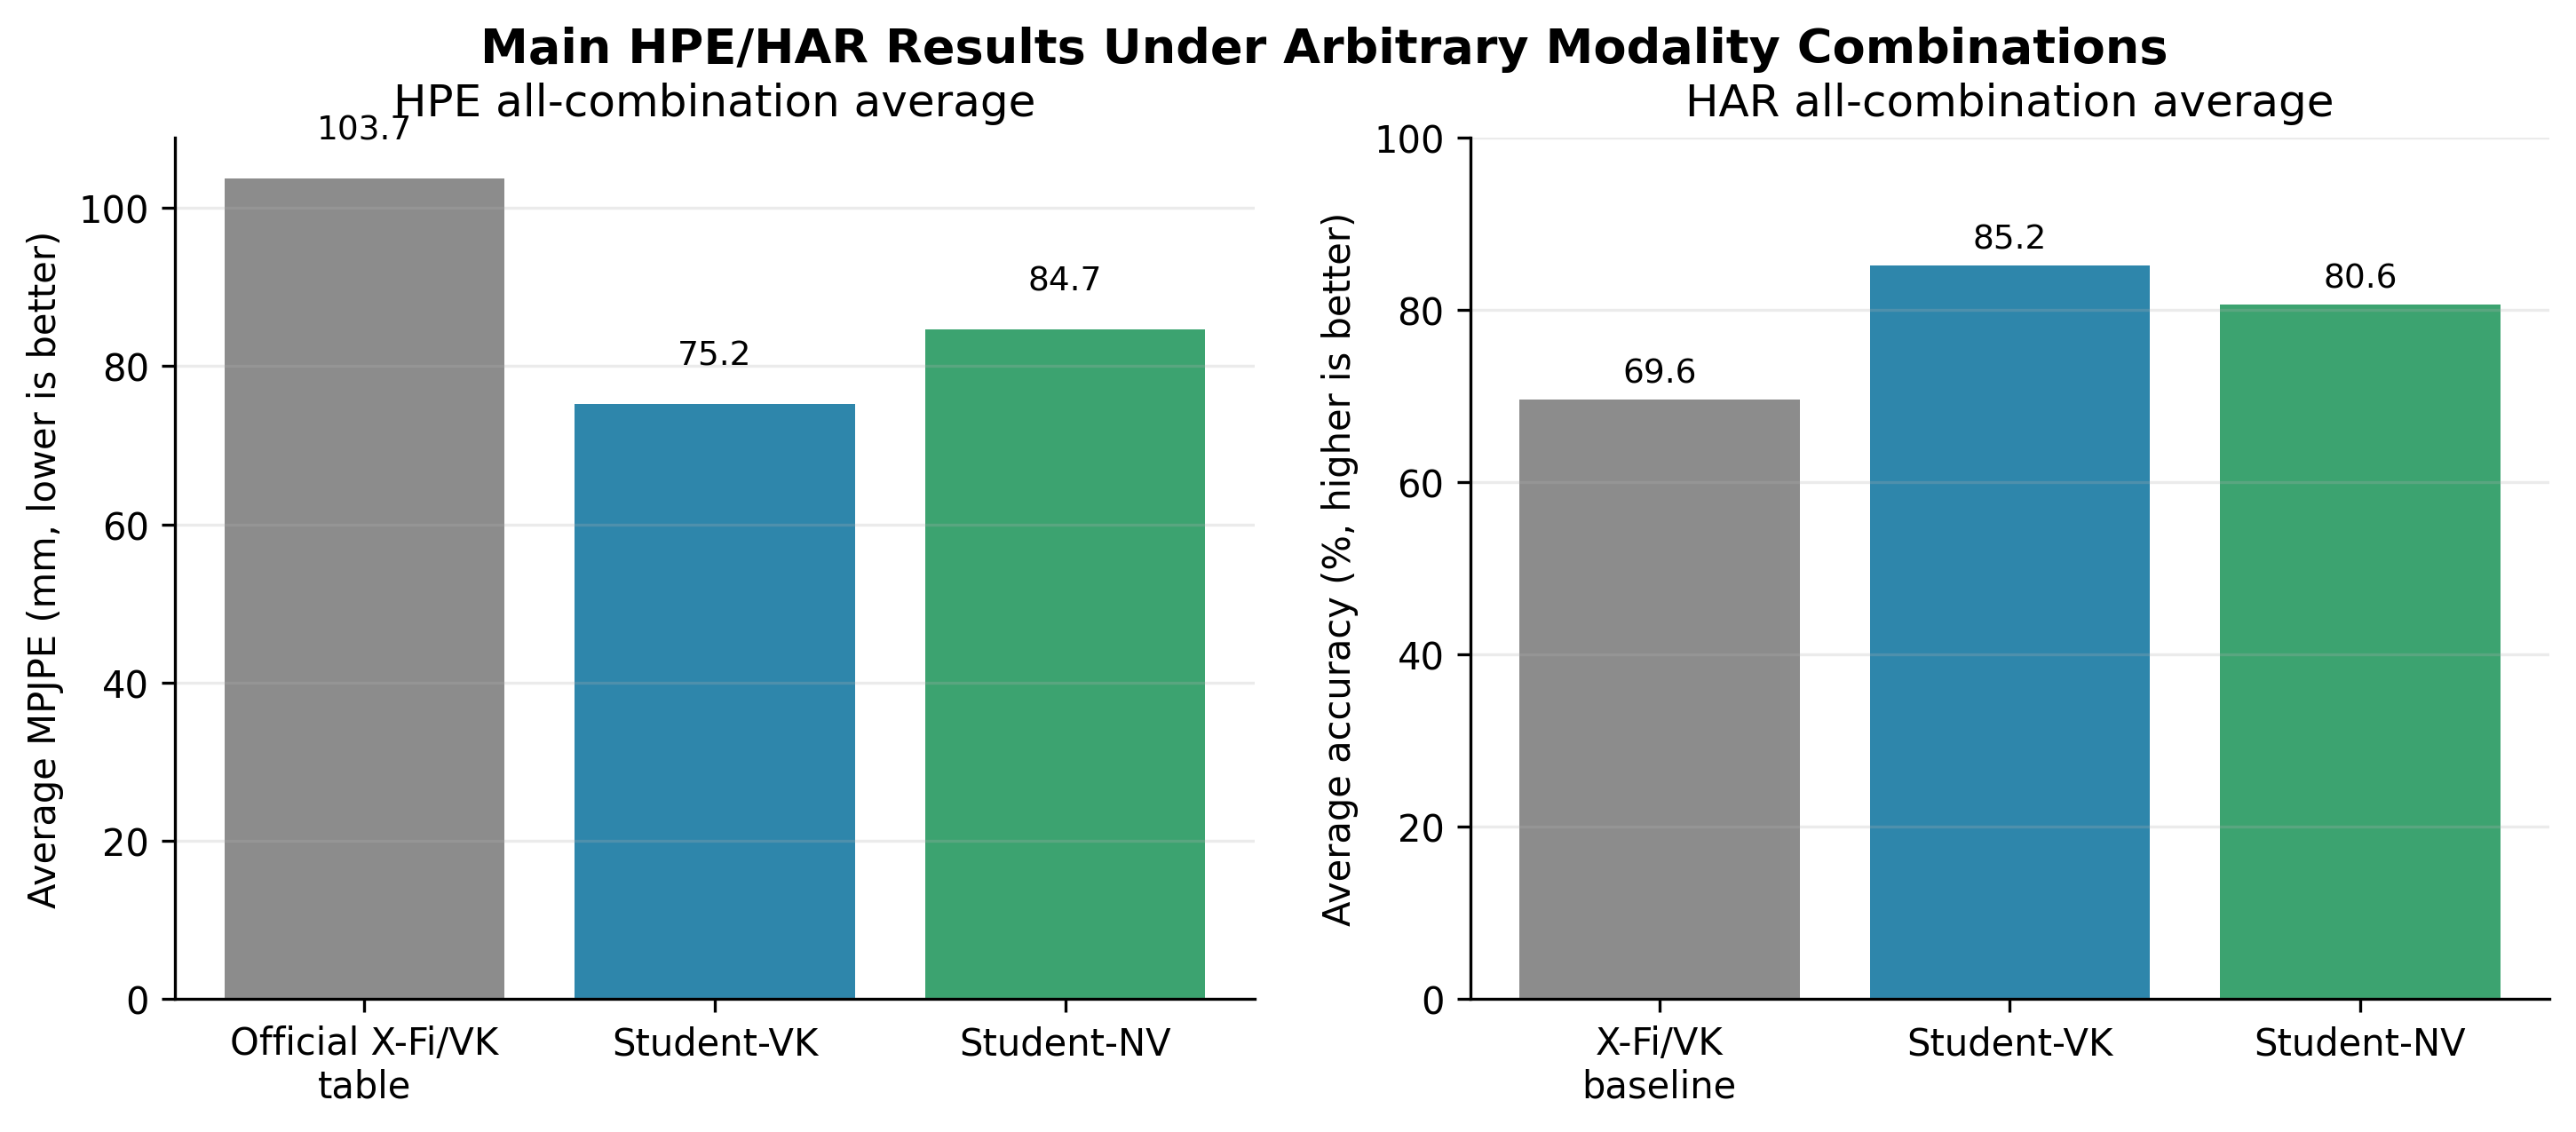
\includegraphics[width=0.92\linewidth]{../figures/fig3_main_results.png}
\caption{Main HPE and HAR results under arbitrary modality combinations. VK-RMD improves the all-combination average over the reproduced X-Fi/VK baseline while supporting deployable non-RGB inference.}
\label{fig:main_results}
\end{figure*}

\subsection{Robustness Under Missing Modalities}

Table~\ref{tab:missing} groups results by the number of missing modalities. For HPE Student-VK, MPJPE increases gradually from 50.17 mm with no missing modality to 124.73 mm when only one modality is available. For HAR Student-VK, accuracy decreases from 96.56\% with all modalities to 70.00\% when only one modality remains. This trend is expected in sensor-sparse IoT conditions and is more informative than reporting only full-modality performance.

\begin{table*}[!t]
\centering
\caption{Grouped missing-modality robustness. HPE values are MPJPE in mm; HAR values are accuracy in percent.}
\label{tab:missing}
\begin{tabular}{lccccc}
\toprule
Task and model & Missing 0 & Missing 1 & Missing 2 & Missing 3 & Missing 4 \\
\midrule
HPE Student-VK & 50.17 & 53.54 & 60.78 & 78.11 & 124.73 \\
HPE Student-NV & 51.03 & 61.32 & 79.43 & 124.32 & -- \\
HAR Student-VK & 96.56 & 93.83 & 87.55 & 70.00 & -- \\
HAR Student-NV & 96.12 & 90.05 & 66.02 & -- & -- \\
\bottomrule
\end{tabular}
\end{table*}

\begin{figure}[!t]
\centering
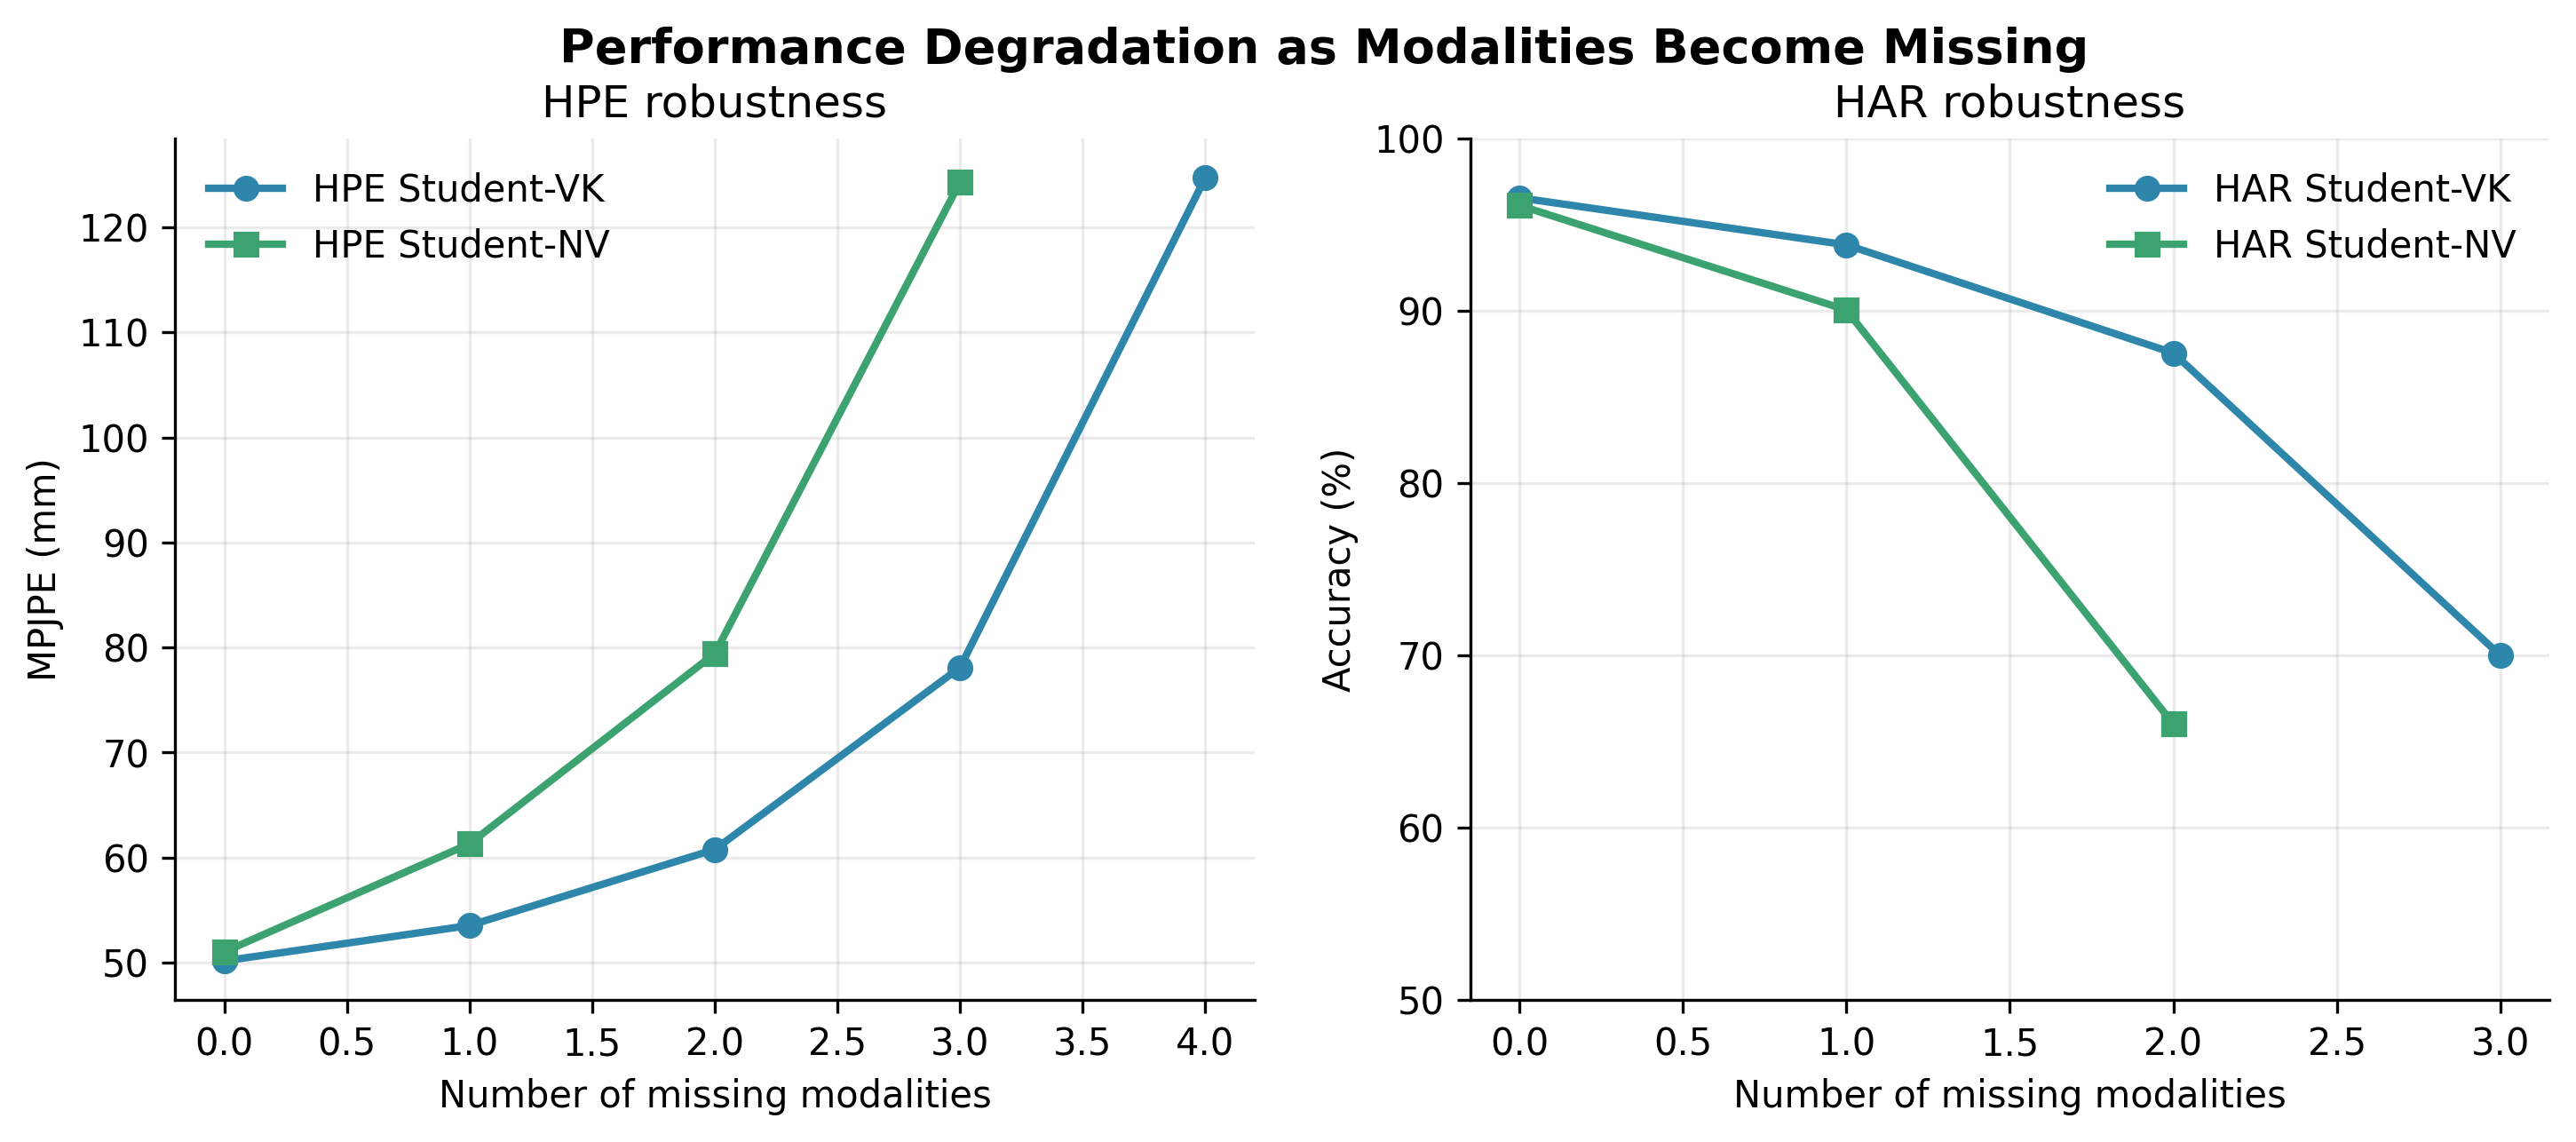
\includegraphics[width=\linewidth]{../figures/fig4_missing_modality_robustness.png}
\caption{Missing-modality robustness comparison. HPE MPJPE increases and HAR accuracy decreases as more sensors are missing, but the Student remains usable under multiple incomplete modality settings.}
\label{fig:missing}
\end{figure}

\subsection{Ablation Study}

Table~\ref{tab:ablation} summarizes the main ablation results. Uniform fusion performs worse than reliability-guided fusion in both tasks. For HPE, uniform fusion obtains 82.77 mm average MPJPE, while VK-RMD Student-VK obtains 75.18 mm. For HAR, uniform fusion obtains 67.46\% average accuracy, while VK-RMD Student-VK obtains 85.15\%. These results support the use of reliability-guided fusion. The no-distillation HPE variant is strong, so the paper does not claim that distillation improves every setting. Instead, distillation is presented as part of the training-time privileged supervision chain, and stronger output-KD evidence should be added before making a broader claim.

\begin{table*}[!t]
\centering
\caption{Ablation results. HPE uses average MPJPE in mm; HAR uses average accuracy in percent. Extreme encoder-ablation failure combinations are not expanded in the main paper.}
\label{tab:ablation}
\begin{tabular}{llccp{2.6in}}
\toprule
Task & Setting & Avg. result & Full result & Interpretation \\
\midrule
HPE & VK-RMD Student-VK & 75.18 & 50.17 & Main HPE model. \\
HPE & w/o distillation & 72.68 & 48.83 & Distillation claim must be cautious for HPE. \\
HPE & uniform fusion & 82.77 & 52.28 & Reliability-guided fusion improves robustness. \\
HAR & VK-RMD Student-VK & 85.15 & 96.56 & Main HAR model. \\
HAR & w/o distillation & 82.86 & 95.99 & Distillation helps HAR average robustness modestly. \\
HAR & uniform fusion & 67.46 & 95.39 & Reliability-guided fusion is important under missing modalities. \\
\bottomrule
\end{tabular}
\end{table*}

\begin{figure*}[!t]
\centering
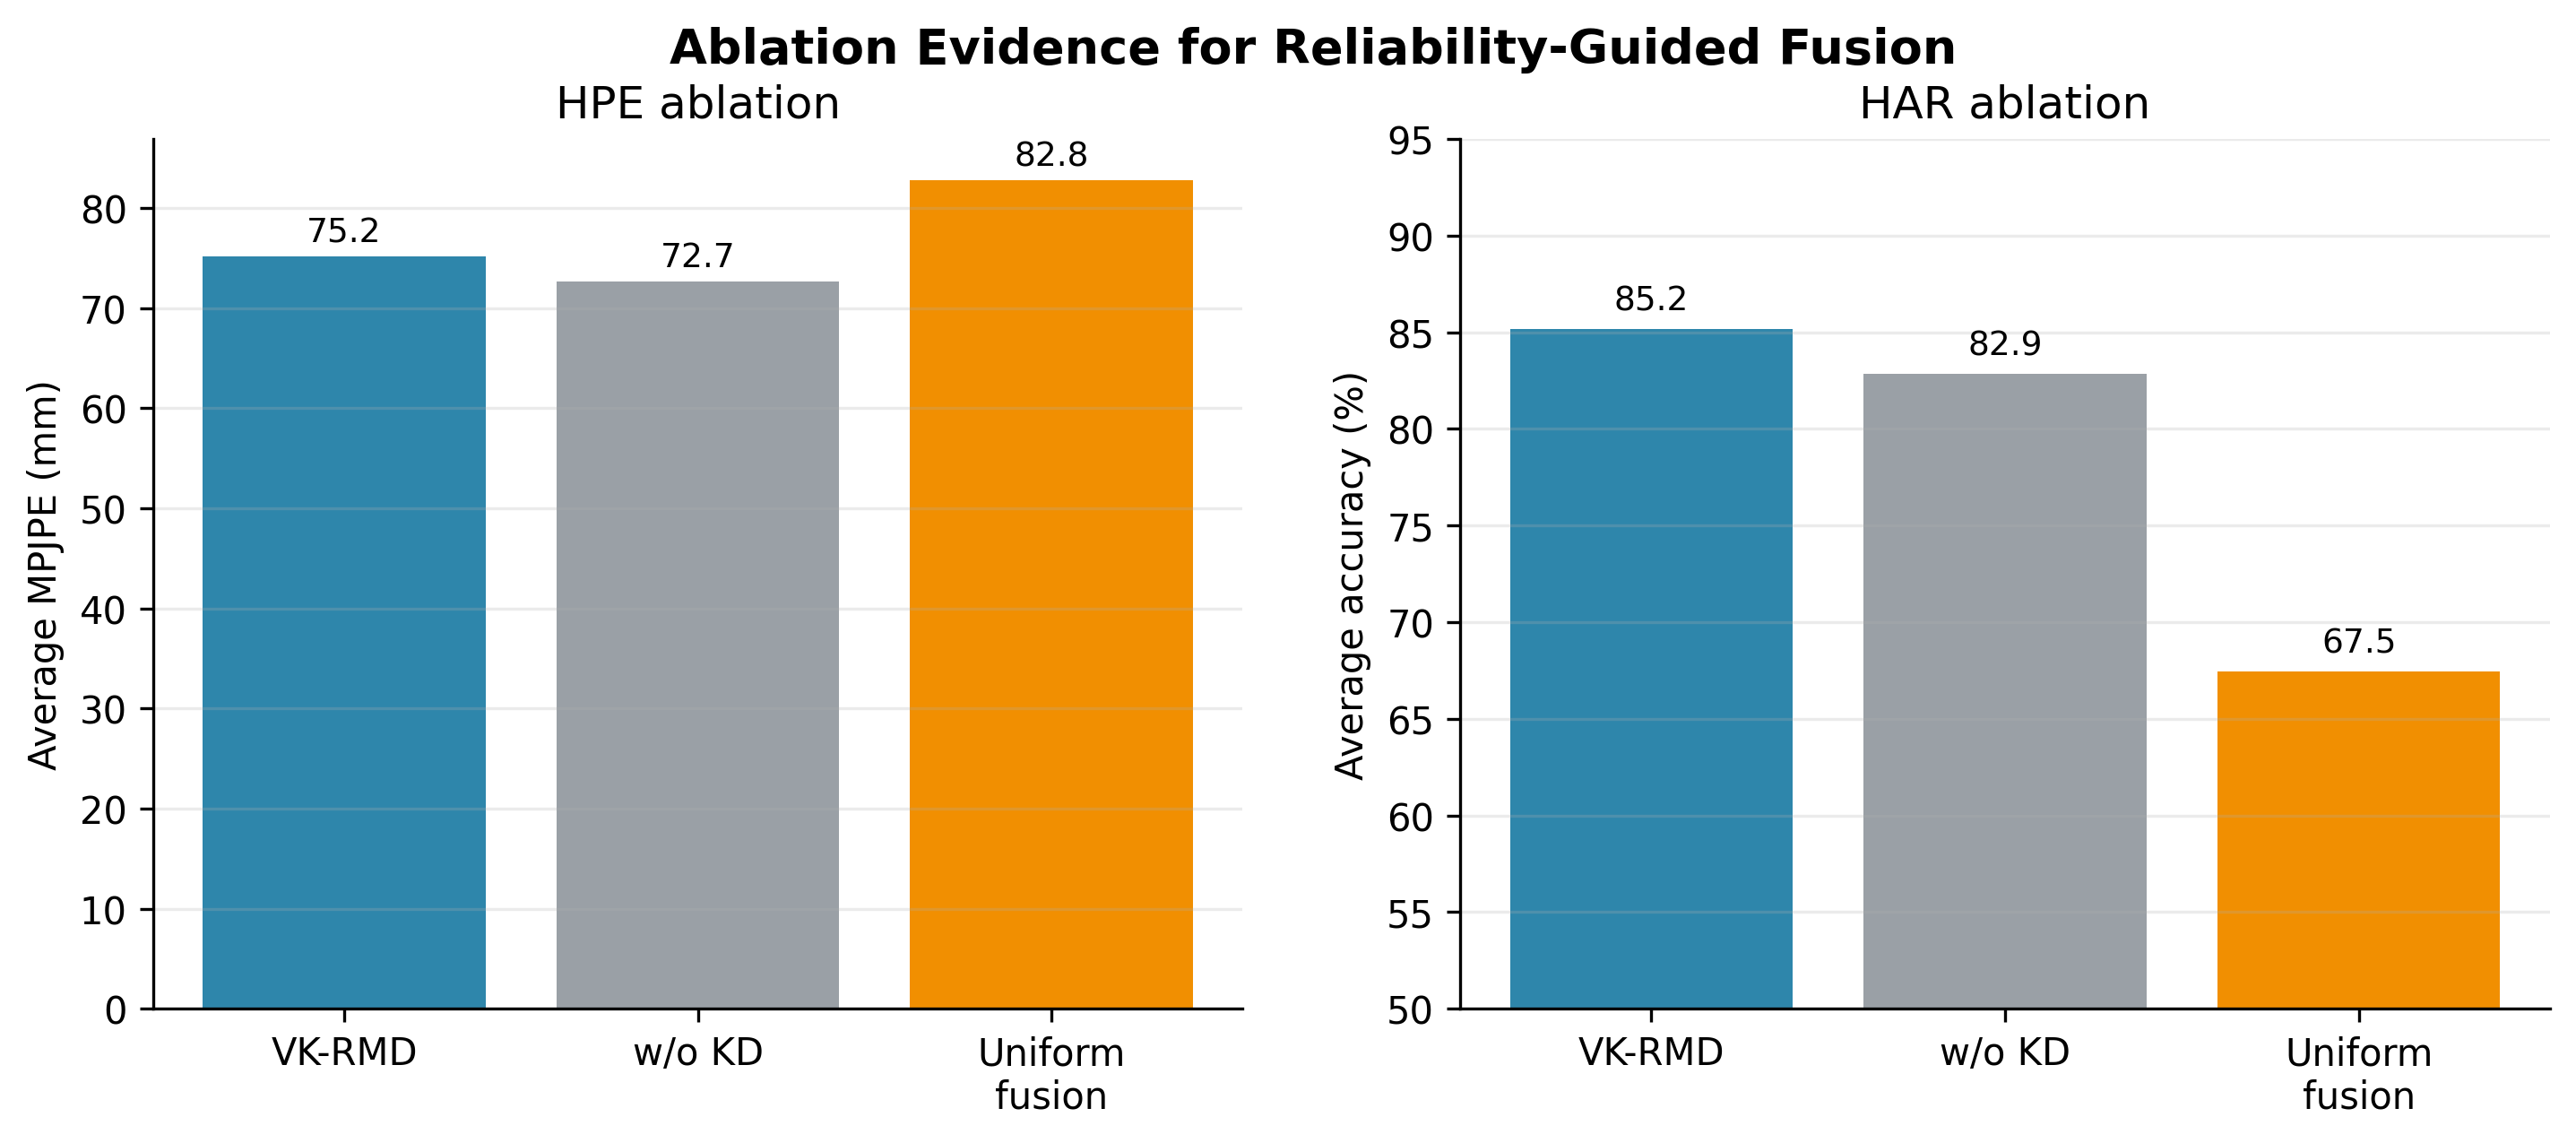
\includegraphics[width=0.92\linewidth]{../figures/fig5_ablation.png}
\caption{Ablation results for the random-split setting. Uniform fusion weakens both HPE and HAR missing-modality robustness, supporting the need for reliability-guided fusion.}
\label{fig:ablation}
\end{figure*}

\subsection{Reliability Weight Analysis}

Fig.~\ref{fig:reliability} directly visualizes the reliability weights learned by VK-RMD. For each modality subset, the weights are normalized over the available modalities, so each row sums to one. In HPE, depth receives the largest average weight in several combinations, such as depth+WiFi-CSI, depth+LiDAR, depth+mmWave, and VK+depth, indicating that the fusion module learns to emphasize geometry-sensitive cues for pose regression. In HAR, mmWave receives larger weights in combinations such as LiDAR+mmWave and VK+mmWave, which is consistent with its motion-sensitive sensing characteristics. These observations support the claim that VK-RMD does not simply average modalities, but adaptively changes decision weights according to the current sensor set and task.

\subsection{Complexity and IoT Deployment Analysis}

Table~\ref{tab:complexity} reports available complexity measurements. The HPE Student-VK and Student-NV models have 8.90M parameters and run above 62 FPS in the measured setting, suggesting feasibility for real-time or near-real-time intelligent-space sensing. FLOPs and HAR runtime should be measured before submission.

\begin{table}[!t]
\centering
\caption{Complexity and deployment-related measurements. Missing entries should be measured before submission.}
\label{tab:complexity}
\begin{tabular}{lccc}
\toprule
Model & Params & FPS & Peak memory \\
\midrule
HPE Student-VK & 8.90M & 62.01 & 4.95 GB \\
HPE Student-NV & 8.90M & 63.37 & 4.95 GB \\
HPE baseline & 5.74M & 52.04 & 4.94 GB \\
HAR Student-VK & 8.61M & To be measured & To be measured \\
\bottomrule
\end{tabular}
\end{table}

\begin{figure}[!t]
\centering
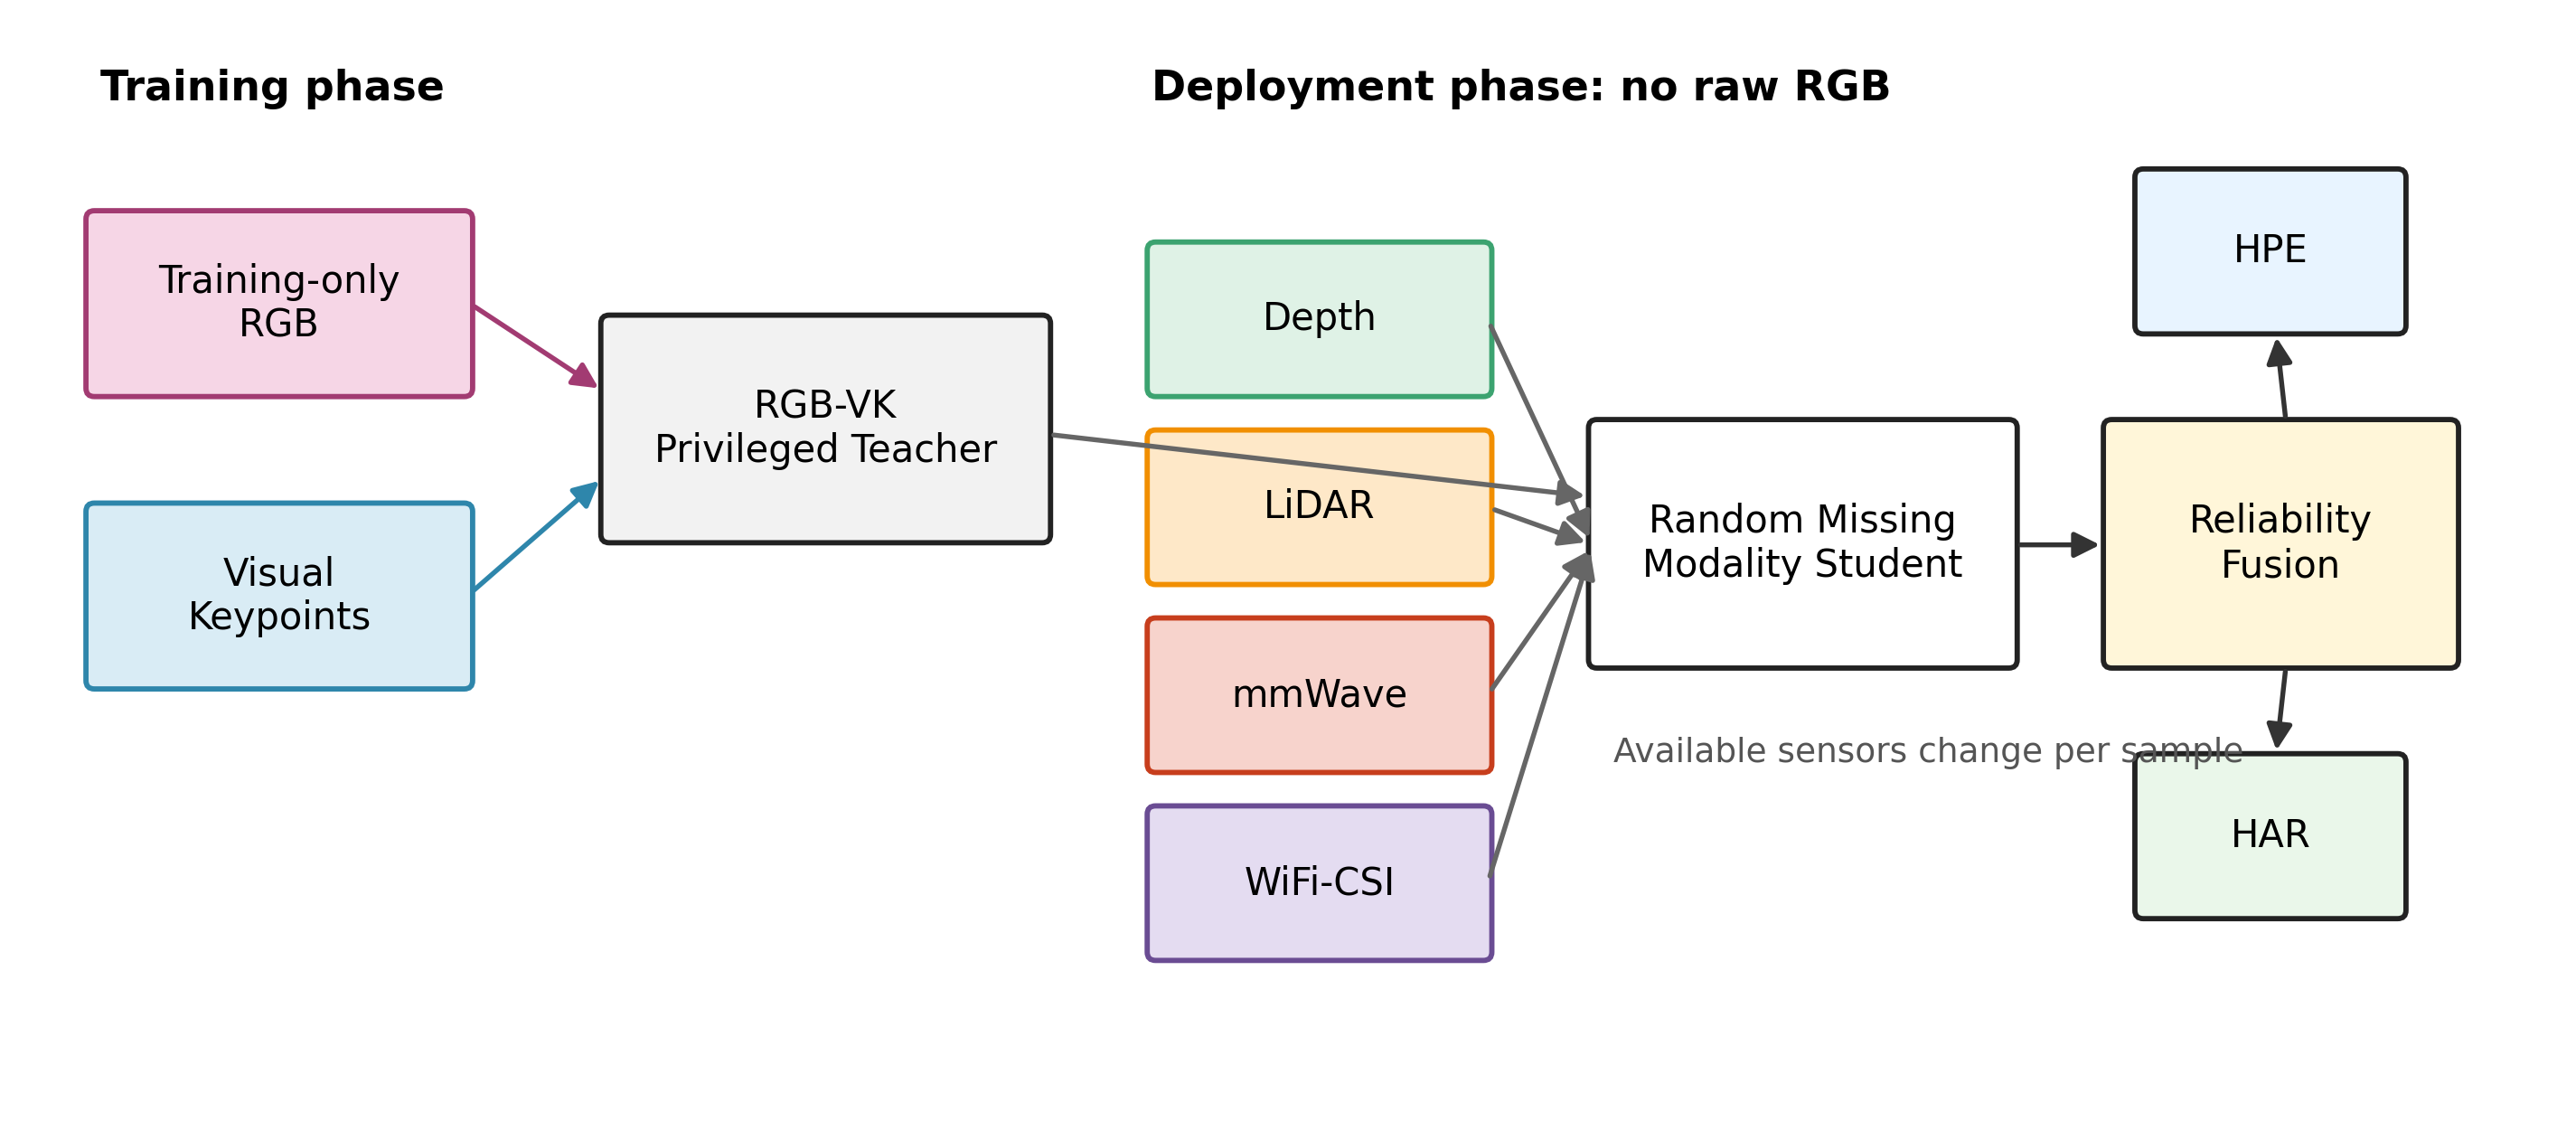
\includegraphics[width=\linewidth]{../figures/fig1_overall_framework.png}
\caption{Teacher-student missing-modality distillation. The teacher uses training-time privileged information, while the deployed Student only consumes available privacy-friendly sensing modalities.}
\label{fig:distill}
\end{figure}

\section{Discussion}

\subsection{Why VK-RMD Fits IoT Intelligent Spaces}

VK-RMD is designed for IoT deployment constraints rather than only benchmark performance. The framework avoids raw RGB at inference, supports heterogeneous non-RGB sensing, and evaluates arbitrary missing-modality combinations. These properties are important for intelligent spaces because installed sensors differ across rooms, users, and applications. A fixed-modality system may be impractical when one sensor is absent or unreliable.

\subsection{Privacy Benefits and Remaining Risks}

The method reduces appearance-level visual exposure by avoiding raw RGB during inference and using VK as a structured bridge. This is more privacy-friendly than camera-centric inference, but it is not a formal privacy guarantee. Body motion, pose, and activity labels can still reveal sensitive behavioral patterns. Therefore, the paper should avoid overstating privacy and should use terms such as privacy-friendly or reduced visual exposure.

\subsection{Limitations}

Several limitations remain. First, the HPE no-distillation ablation is competitive, so the distillation contribution should be stated carefully and strengthened with output-KD combination results. Second, the reliability weights provide interpretability at the modality level, but they do not constitute a causal proof that a sensor is always more informative in every environment. Third, the exploratory SuperTeacher results are not strong enough to be presented as a main contribution; they should remain in discussion or appendix. Fourth, real-world IoT deployment with live sensors remains future work.

\subsection{Future Work}

Future work should extend VK-RMD to streaming deployment, online sensor-quality estimation, edge-device acceleration, and stronger privacy analysis. Additional experiments should measure runtime on edge hardware and evaluate robustness under real sensor failures rather than only offline modality masking.

\section{Conclusion}

This paper presented VK-RMD, a privacy-friendly and missing-modality robust multimodal human sensing framework for IoT-enabled intelligent spaces. RGB is used as training-time privileged information, VK acts as a structured bridge, and the deployed Student operates without raw RGB. Through random missing-modality training and reliability-guided fusion, VK-RMD supports HPE and HAR under arbitrary available sensor combinations. Experiments on MMFi show strong HPE and HAR performance under random, cross-scene, and cross-subject protocols. The results support VK-RMD as a practical direction for sensor-availability-aware human perception in privacy-sensitive IoT spaces.

\begin{thebibliography}{35}

\bibitem{mmfi}
Y. Yang \emph{et al.}, ``MMFi: Multi-modal non-intrusive 4D human dataset for versatile wireless sensing,'' \emph{to be verified before submission}.

\bibitem{xfi}
NTUMARS, ``X-Fi: Modality-invariant multimodal human sensing,'' \emph{to be verified before submission}.

\bibitem{lupi}
V. Vapnik and A. Vashist, ``A new learning paradigm: Learning using privileged information,'' \emph{Neural Networks}, 2009, to be verified.

\bibitem{kd}
G. Hinton, O. Vinyals, and J. Dean, ``Distilling the knowledge in a neural network,'' arXiv:1503.02531, 2015.

\bibitem{openpose}
Z. Cao, G. Hidalgo, T. Simon, S.-E. Wei, and Y. Sheikh, ``OpenPose: Realtime multi-person 2D pose estimation using part affinity fields,'' \emph{IEEE TPAMI}, to be verified.

\bibitem{stgcn}
S. Yan, Y. Xiong, and D. Lin, ``Spatial temporal graph convolutional networks for skeleton-based action recognition,'' in \emph{AAAI}, 2018, to be verified.

\bibitem{missing_survey}
Author, ``Missing-modality robust multimodal learning: A survey,'' \emph{to be verified}.

\bibitem{multimodal_fusion_survey}
Author, ``Multimodal sensor fusion for human activity recognition: A survey,'' \emph{to be verified}.

\bibitem{privacy_sensing}
Author, ``Privacy-preserving human sensing in smart environments,'' \emph{to be verified}.

\bibitem{iot_sensing}
Author, ``Human-centric sensing in Internet of Things environments,'' \emph{to be verified}.

\bibitem{edge_intelligence}
Author, ``Edge intelligence for IoT sensing systems,'' \emph{to be verified}.

\bibitem{wifi_har}
Author, ``WiFi CSI-based human activity recognition,'' \emph{to be verified}.

\bibitem{mmwave_har}
Author, ``mmWave radar for human activity recognition,'' \emph{to be verified}.

\bibitem{lidar_human}
Author, ``LiDAR-based human perception,'' \emph{to be verified}.

\bibitem{depth_hpe}
Author, ``Depth-based human pose estimation,'' \emph{to be verified}.

\bibitem{hpe_survey}
Author, ``Human pose estimation: A survey,'' \emph{to be verified}.

\bibitem{har_survey}
Author, ``Human activity recognition: A survey,'' \emph{to be verified}.

\bibitem{modality_dropout}
Author, ``Modality dropout for multimodal learning,'' \emph{to be verified}.

\bibitem{reliability_fusion}
Author, ``Reliability-aware multimodal fusion,'' \emph{to be verified}.

\bibitem{attention_fusion}
Author, ``Attention-based multimodal fusion,'' \emph{to be verified}.

\bibitem{cross_modal_distill}
Author, ``Cross-modal knowledge distillation for sensor-based perception,'' \emph{to be verified}.

\bibitem{privileged_distill}
Author, ``Privileged distillation for multimodal perception,'' \emph{to be verified}.

\bibitem{smart_home}
Author, ``Smart home sensing systems for assisted living,'' \emph{to be verified}.

\bibitem{health_monitoring}
Author, ``IoT-based health monitoring using human sensing,'' \emph{to be verified}.

\bibitem{human_robot}
Author, ``Human-aware perception for embodied intelligence,'' \emph{to be verified}.

\bibitem{wireless_pose}
Author, ``Wireless sensing for human pose estimation,'' \emph{to be verified}.

\bibitem{csi_pose}
Author, ``CSI-based human pose estimation,'' \emph{to be verified}.

\bibitem{radar_pose}
Author, ``Radar-based human pose estimation,'' \emph{to be verified}.

\bibitem{sensor_dropout}
Author, ``Robust IoT sensing under sensor dropout,'' \emph{to be verified}.

\bibitem{multitask_hpe_har}
Author, ``Joint human pose estimation and action recognition,'' \emph{to be verified}.

\bibitem{graph_skeleton}
Author, ``Graph-based skeleton representation for human action recognition,'' \emph{to be verified}.

\bibitem{transformer_sensor}
Author, ``Transformer models for multimodal sensor perception,'' \emph{to be verified}.

\bibitem{domain_generalization}
Author, ``Domain generalization for human sensing,'' \emph{to be verified}.

\bibitem{cross_scene}
Author, ``Cross-scene evaluation for intelligent-space sensing,'' \emph{to be verified}.

\bibitem{efficient_iot}
Author, ``Efficient neural models for IoT edge deployment,'' \emph{to be verified}.

\end{thebibliography}

\end{document}
